\section{Extruding PLCL Discussion\label{discussion:extrudingPLCL}}

\subsection{Qualitatively Assessing Filament Output\label{discussion:extrudingPLCL:assessingFilamentOutput}}

\hl{Add what I look for in terms of filament quality with a table as well}.

\subsection{Powder Extrusion Discussion\label{sec:discussion:extrudingPLCL:powderExtrusion}}

While this extrusion was successful in that filament was extruded, the extruded filament was unusable. When evaluating filament quality from a 3D printable perspective, there are numerous factors that must be considered (see~\fullref{sec:literatureReview:extrusion:issues} for a detailed explanation of these factors).

\paragraph*{Filament Output}
The filament was highly brittle and could snap easily. Although the powder was dried prior to extrusion and allowed to cool in air, brittleness was still a significant concern. This is the third extruder the team has used for powder extrusions (see~\fullref{sec:introduction:priorWork:otherTeamWork:plclExtrusions} for more information) and all three extruders led to highly brittle output. As a result, it is hypothesized at this point that a fully powder-based extrusion may create unusably brittle filament.

Additionally, the output was thin and experienced a variable flow rate. The Devostick pusher was used to address feed rate variability, but this did not adequately solve the issue. The variable feed rate and Devostick also led to concerning spikes in current as shown in~\autoref{fig:results:extrudingPLCL:powderExtrusion:currentOutput}.

Lastly, the filament had air bubbles inside indicative of temperature being too high. If the temperature is too high, the powder is likely degrading into a gas~\cite{RefWorks:RefID:396-3devotroubleshooting}. These air bubbles are shown below in~\autoref{fig:results:extrudingPLCL:powderExtrusion:airBubbles}

\begin{figure}[h!]
        \centering
        \includegraphics[width=0.3\linewidth]{../figs/discussion/plclExtrusions/powderExtrusion/air_bubbles.png}
        \caption{Performing PLCL powder extrusion. Measuring powder (left) and pouring into extruder (right).}
        \label{fig:results:extrudingPLCL:powderExtrusion:airBubbles}
\end{figure}

\paragraph*{Alternative Approaches}

Based on significant time dedicated to powder-based PLCL extrusions starting on Felfil and Filabot systems (see~\fullref{sec:introduction:priorWork:otherTeamWork:plclExtrusions}) and the lack of successfully extruding PLCL filament, the research team decided to explore alternative approaches in case powder-based extrusions remained unsuccessful.

Various alternative device development approaches were researched including embedded 3D printing, multi-material 3D printing, and hydrogels (see~\fullref{sec:literatureReview:alternativeDevices}). Various project road mapping techniques were also explored and tested (see~\fullref{sec:literatureReview:roadmap}).

\paragraph*{Extrusion Process}

In addition to the filament output, there were concerns with the extrusion process as a whole. It was noted that the powder formed clumps (bridging) at the hopper. Even with the Devostick pusher, these clumps could not be consistently broken up which contributed to the variable flow rate. It was determined based on feedback from 3Devo customer support that this clumping is likely due to solely using powders and the heat zone temperatures being too high.

Also, the process of extruding powder was found to be chaotic and messy as well as inefficient. It was difficult to keep the powder from dispersing when transferring from the initial container to the hopper. This led to dirtying of equipment and wasted raw material.

\paragraph*{Key Takeaways}
% order feeder, powders will always be brittle
Key takeaways from this extrusion experiment are that: a 3Devo Feeder~\cite{RefWorks:RefID:310-3devofeeder} should be ordered to address clumping and variable flow rate, heat zones should be decreased to address clumping, cleaning supplies should be ordered to address powder dispersion, and alternative extrusion routes should be explored to address inherent brittleness of powder extrusions.

Because the Nomisma PLCL powder is expensive and has a long lead time, the team decided to pause powder extrusion research until the 3Devo Feeder arrived to avoid potentially wasting raw material. In the meantime, alternative device fabrication approaches were explored.

\subsection{Pellet Extrusions Discussion\label{sec:discussion:extrudingPLCL:pelletExtrusions}}

\subsubsection{Combining Materials Discussion\label{sec:discussion:extrudingPLCL:pelletExtrusions:combiningMaterials}}

As mentioned in ~\fullref{sec:methodology:extrudingPLCL:pelletExtrusions:combiningMaterials}, various methods were explored to combine PLA and PCL pellets into a homogenous mixture.

\paragraph*{College of Pharmacy}

It was determined that the College of Pharmacy did not have adequate equipment to assist in mixing PLA and PCL pellets. Any mixing equipment they were able to provide was meant for small-scale (a few gram) mixing.

\paragraph*{Injection Molding}

While injection molding was deemed a possible option for combining these materials, it was eventually ruled out based on limitations of the equipment and the research team.

Discussions with professors at Ohio State University as well as a review of relevant literature made it apparent that injection molders could combine materials but would not reliably mix the materials homogeneously.

Various faculty were also hesitant to recommend injection molding given the steep learning curve and high setup time required to operate the equipment.

\paragraph*{Chemically Combining Materials}

After discussing the option of chemically combining the pellets with the PSRF (see~\autoref{sec:methodology:externalLabs:polymersLab}) using chloroform or DCM as a dissolving agent, the team was told this could not be done. For safety purposes, the PSRF no longer carries DCM or chloroform and is not allowed to work with these materials in most cases.

The final output of thermally combining the materials on a hotplate, as shown in~\autoref{fig:methodology:extrudingPLCL:meltingOnHotplate}, was too large to easily shred into extrudable pellets. Melting these materials in a shallower and wider dish may have resulted in a more shreddable output. However, this could not be done easily on a hotplate for the scale of materials needed for extruding. As a result, this rudimentary method of combining materials was eliminated.

\paragraph*{3D Printable Mixing Systems}

The research team decided that 3D printable tumbler systems were usable for mixing materials but that it may require more time than expected to fully assemble these systems. The team felt that if dedicated mixing equipment was required, this would be the fastest and cheapest approach. However, the team wanted to first see if they needed dedicated mixing equipment at all before spending time and resources in building these systems.

\paragraph*{Discussions with ISE Department}

Discussions with the ISE department were helpful in planning out multiple best and worst-case options for mixing materials given available equipment, time, and material constraints.

Dr. Mulyana was confident that dedicated mixing equipment was not required and that the pellets could be manually mixed in a container prior to extrusion. Due to a single screw extruder's inherently poor mixing capabilities, the limiting factor in creating a homogenous output would be the extruder rather than the degree of homogeneity of the pre-extrusion mixture.

To address this bottleneck, Dr. Mulyana offered the team uses a twin screw extruder in the ISE department. While this equipment would mix materials well, it would require high volumes of raw materials to run and time to learn how to use this equipment. It was decided that a twin screw extruder would be a viable backup option if using a single screw extruder did not mix materials well enough.

\paragraph*{Key Takeaways}

Many options were explored to combine PLA and PCL pellets into a homogenous mixture prior to extruding. Based on time, cost, safety, and anticipated limitations of equipment, injection molding, combining materials in a lab setting, and 3D printing a mixing system were no longer explored.

After consulting with Dr. Mulyana, the team opted to start by mixing pellets manually in a jar, leaving other methods for later consideration.

\subsubsection{Initial Pellet Extrusion Discussion\label{sec:discussion:extrudingPLCL:pelletExtrusions:initialPelletExtrusion}}

The team was surprised that this extrusion led to clumping at the hopper given the use of the Feeder and pellets rather than powders. The expected outcome of using the Feeder was that its vibrations would keep pellets from being stagnant long enough to start bridging.

Conversations with 3Devo customer support following this extrusion revealed that the Feeder can not be used with more than one homogenous material. When a blend is poured into the hopper, the Feeder's vibrations will cause solid segregation, causing one material to sink to the bottom and the other to rise to the top. This was directly seen in the extrusion with PLA moving to the bottom of the hopper and PCL moving to the top.

It was expected that temperatures were low enough to prevent premature melting of material. However, PCL pellets appeared to melt and bridge in the hopper. 3Devo customer support believed this is because the metal hopper is not insulated, so material sitting in the hopper for extended periods of time can be subject to additional heat. Because PCL has a lower melting point than PLA, the PLA pellets did not melt while sitting in the hopper but the PCL pellets began to.

As a result, it was recommended to explore PCL's workable extrusion temperature range to determine how high temperatures could be set for this material. Ideally the upper end of the PCL extrusion temperature range would overlap with the lower end of the PLA extrusion temperature range. This overlap would be the ideal extrusion temperature for the blend of materials.

Starve feeding, or pouring material directly into the barrel rather than letting it sit in the hopper, was suggested to prevent PCL from prematurely melting in the uninsulated metal hopper. It was also hypothesized that insulating the hopper could help prevent this premature melting.

\paragraph*{Key Takeaways}

This extrusion helped drive research forward by highlighting new concerns with multi-material pellet extrusions. It was found that the Feeder could not be used on blends of materials and PCL could not sit in the metal hopper for extended periods of time without beginning to soften and melt.

Based on this extrusion, the next steps were to extrude PCL alone and determine its working extrusion temperature range.

\subsubsection{PCL Temperature Study Discussion\label{sec:discussion:extrudingPLCL:pelletExtrusions:pclTempStudy}}

Based on the rise in current at 60-80\textcelsius, ~3Devo customer support hypothesized that the PCL was too solid and forming a clog inside the barrel. As a result, PCL should not be extruded below 80\textcelsius.

No issues were seen with feeding or filament output between 80\textcelsius ~and 150\textcelsius. Premature melting began at 160\textcelsius. Filament output was still consistent at these higher temperatures, but starve feeding had to be more closely monitored to prevent bridging at the hopper.

Figure~\ref{fig:discussion:extrudingPLCL:pelletExtrusions:pclTempRange} illustrates the working temperature range for PCL pellets based on this temperature study.

\begin{figure}[h!]
        \centering
        \includegraphics[width=\linewidth]{../figs/discussion/plclExtrusions/pelletExtrusions/pcl_extrusion_temperature_range.png}
        \caption{PCL working extrusion temperature range.}
        \label{fig:discussion:extrudingPLCL:pelletExtrusions:pclTempRange}
\end{figure}

Based on this extrusion study, PCL should ideally be extruded between 80 and 150\textcelsius, ~but can be extruded as high as 180\textcelsius ~as long as starve feeding is closely monitored.

\subsubsection{Manual Starve Feeding Discussion\label{sec:discussion:extrudingPLCL:pelletExtrusions:manualStarveFeeding}}

Given the susceptibility of PCL to clog at temperatures above 160\textcelsius, ~starve feeding must be closely monitored when extruding at these temperatures.  When performing all starve feeding manually, the researcher is unable to move away from the extruder due to the short time between starve feeding sessions. It was found that starve feeding was required roughly every two minutes or less and at precise amounts. Because extrusions often last multiple hours, manual starve feeding is not an efficient or sustainable process.

As a result, an automatic starve feeding system should be developed to assist with starve feeding.

\subsubsection{Initial PLCL Extrusion with Starve Feeder Discussion\label{sec:discussion:extrudingPLCL:pelletEtrusions:initialStarveFeederExtrusion}}

\paragraph*{Success of Extrusion}

While the filament thickness was variable and overall too thin, this extrusion achieved a notable milestone for the research team. This was the first time the research was able to steadily extrude good-quality PLCL filament (no air bubbles and not overly brittle).

This extrusion proved the efficacy of the starve feeder given the improvements in extrusion output rate and lack of clogging from the initial PLCL extrusion (see~\fullref{sec:methodology:sec:discussion:extrudingPLCL:pelletExtrusions:initialPelletExtrusion}).

\paragraph*{Filament Thickness}

The thickness of the spooled filament was a concern created by this extrusion. Although good-quality filament was being output from the nozzle, spooling at a proper thickness (1.65mm to 1.85mm) is a requirement of creating 3D printable filament. Thus, the thickness tolerance needed to be improved to be able to attempt printing this custom filament.

The research team was unsure why the output filament was unable to be spooled at a consistent thickness, and decided to discuss these concerns with 3Devo customer support.

3Devo customer support suggested this thin filament indicated the material needed to stay more solidified early on to help push out material faster. It was suggested to lower heater 4, the heater closest to the hopper, to try and keep the material more solidified for longer.

It was also hypothesized that contaminants inside the extrusion barrel could be causing this variable output. A full purge of the extruder was recommended to clean the extruder barrel of any potential contaminants.

\paragraph*{Key Takeaways}

This was the first successful PLCL extrusion for the team. Manually combining PLA and PCL pellets and dispensing material directly into the extruder barrel using the automatic starve feeder proved a functional way to extrude PLCL filament.

The thickness of the spooled filament was highly variable and on average too thin which likely means the extrusion parameters (heat zones and RPM) need to be adjusted.

\subsubsection{Addressing Filament Thickness Discussion\label{sec:discussion:extrudingPLCL:pelletExtrusions:addressingFilamentThickness}}

\paragraph*{Adjusting Heat Zones}

After numerous heat zone adjustments, the spooled filament thickness of the PLA/PCL extrusion was still too thin. 3D printers require tight tolerances (often 1.75±0.03mm) which these extrusions were not within.

Suggestions from 3Devo customer support included lowering heat zones 4 and 3 and raising extruder screw RPM, but when that was not working they did not have many new suggestions.

Because the heat zone adjustment was not yielding adequate results, 3Devo customer support suggested more routinely purging the extruder in case contaminants were blocking the flow of material. They also suggested replacing the standard 4mm nozzle with a 2mm nozzle. As a result, purging compounds were explored (see ~\fullref{sec:methodology:extrudingPLCL:purgingExtruder}) and a smaller nozzle was ordered from 3Devo~\cite{RefWorks:RefID:392-3devo}.

Since the nozzle had to be ordered from 3Devo which required international shipping, it was assumed this would have a substantial lead time. Therefore, alternative extrusion options were explored while waiting for a smaller nozzle to arrive (see ~\fullref{sec:methodology:extrudingPLCL:felfilSystem}).

\paragraph*{Extruding PLCL Regrind}

The PLCL regrinding extrusion yielded promising results in that the initial output was much thicker visually than the first-pass PLCL. Unfortunately, thickness readings could not be measured due to an issue with 3Devo's DevoVision software. Newer computers were bought and updated software had been downloaded following this initial regrind extrusion to resolve these issues.

Once the DevoVision software was functioning properly again, the research team attempted to perform more PLCL regrind extrusions. While this was attempted multiple times, clogging and unfinished purges inhibited this process. This led to additional research into purging the extruder (see ~\fullref{sec:methodology:extrudingPLCL:purgingExtruder}).

\paragraph*{Clogged Extruder}

It was noticed that the extruder routinely formed a clog when shifting from low temperature PLA/PCL extrusions to PLA at normal PLA presets. Due to a limited supply of purging compounds, PLA was run in the extruder until this clog was resolved. This ended up being a time and material intensive process.

As a result, 3Devo customer support recommended properly purging the extruder after every extrusion. This led to additional research into purging the extruder (see ~\fullref{sec:methodology:extrudingPLCL:purgingExtruder}).

\paragraph*{Key Takeaways}

Multiple extrusion attempts were performed to refine the filament thickness following the initial successful PLCL extrusion. Heat zones and RPM were adjusted and first-pass PLCL extrusion was shredded and re-extruded. Various sized extruder nozzles were ordered to address the overall filament thickness.

Extruding reground filament appeared to help the overall filament thickness, but data could not be collected due to issues with DevoVision software. Subsequent regrind extrusions were performed but clogging in the extruder and improper purging procedures inhibited these experiments. As a result, purging procedures and compounds were further researched (see ~\fullref{sec:methodology:extrudingPLCL:purgingExtruder}).

\subsection{Purging 3Devo Extruder Discussion\label{sec:discussion:extrudingPLCL:pelletExtrusions:purgingExtruder}}

\subsubsection{Initial Purging Process Discussion\label{sec:discussion:extrudingPLCL:pelletExtrusions:purgingExtruder:initialPurge}}

The initial DevoClean MT output contained substantial contaminants at first and then transitioned to fully clean purging material. This high level of contamination within the barrel made it clear that regular purging is necessary for consistent extruding.

As mentioned earlier, however, limited supply of 3Devo's DevoClean MT remained which resulted in infrequent purging. $1kg$ of material was provided with the extruder purchase, and roughly $\frac{1}{3}kg$ of material is used with every purge.

This led to a deeper exploration of available purging materials as described in \fullref{sec:methodology:extrudingPLCL:purgingExtruder:supplierDiscovery}.

\subsubsection{Purging with DP-L Discussion\label{sec:discussion:extrudingPLCL:pelletExtrusions:purgingExtruder:dpLPurge}}

\paragraph*{Benefits of DP-L Over DevoClean MT}

The largest benefit of using DP-L as an extruding compound rather than DevoClean MT was not having to use HDPE to transition between materials. Additionally, DP-L used less material and acted faster than DevoClean MT.

\paragraph*{Efficacy of DP-L}

Purging with DP-L initially appeared successful. The output was similar to a DevoClean MT purge in that contaminated output transitioned to clean purging material.

However, when performing subsequent extrusions following a DP-L purge, black specks were noticed in the extrusion output as shown below in Figure~\ref{fig:sec:discussion:extrudingPLCL:pelletExtrusions:purgingExtruder:dpLBlackSpecks}.

\begin{figure}[h!]
        \centering
        \includegraphics[width=0.5\linewidth]{../figs/discussion/purgingExtruder/dpL_purge_black_specks.png}
        \caption{Black specks noticed following a DP-L purge. Initially small specks (A) that became larger (B).}
        \label{fig:sec:discussion:extrudingPLCL:pelletExtrusions:purgingExtruder:dpLBlackSpecks}
\end{figure}

Following discussions with 3Devo customer support and Dyna-Purge customer support, it was believed that these specks were indicative of contaminants left inside the barrel. This means that DP-L was not effectively cleaning the inside of the barrel when purging the extruder.

As a result, DP-D2 was tested due to its closer MFI to PLA and more effective cleaning abilities per Dyna-Purge customer support (see Section~\ref{sec:methodology:extrudingPLCL:purgingExtruder:dpD2Purge}).

\paragraph*{Key Takeaways}

While DP-L purged faster and using less material than DevoClean MT, it was found to ineffectively clean all contaminants in the extruder. These findings led to exploring DP-D2 as a purging compound based on Dyna-Purge's recommendation.

\subsubsection{Purging with DP-D2 Discussion\label{sec:discussion:extrudingPLCL:pelletExtrusions:purgingExtruder:dpD2Purge}}

\paragraph*{Efficacy of DP-D2}
Using DP-D2 as opposed to DP-L for purging the extruder initially appeared successful. the contaminants in the output filament following a purge mostly disappeared. The contaminants still appeared in output filament, though in much smaller quantities as shown in Figure~\ref{fig:sec:discussion:extrudingPLCL:pelletExtrusions:purgingExtruder:dpd2BlackSpecks}.

\begin{figure}[h!]
        \centering
        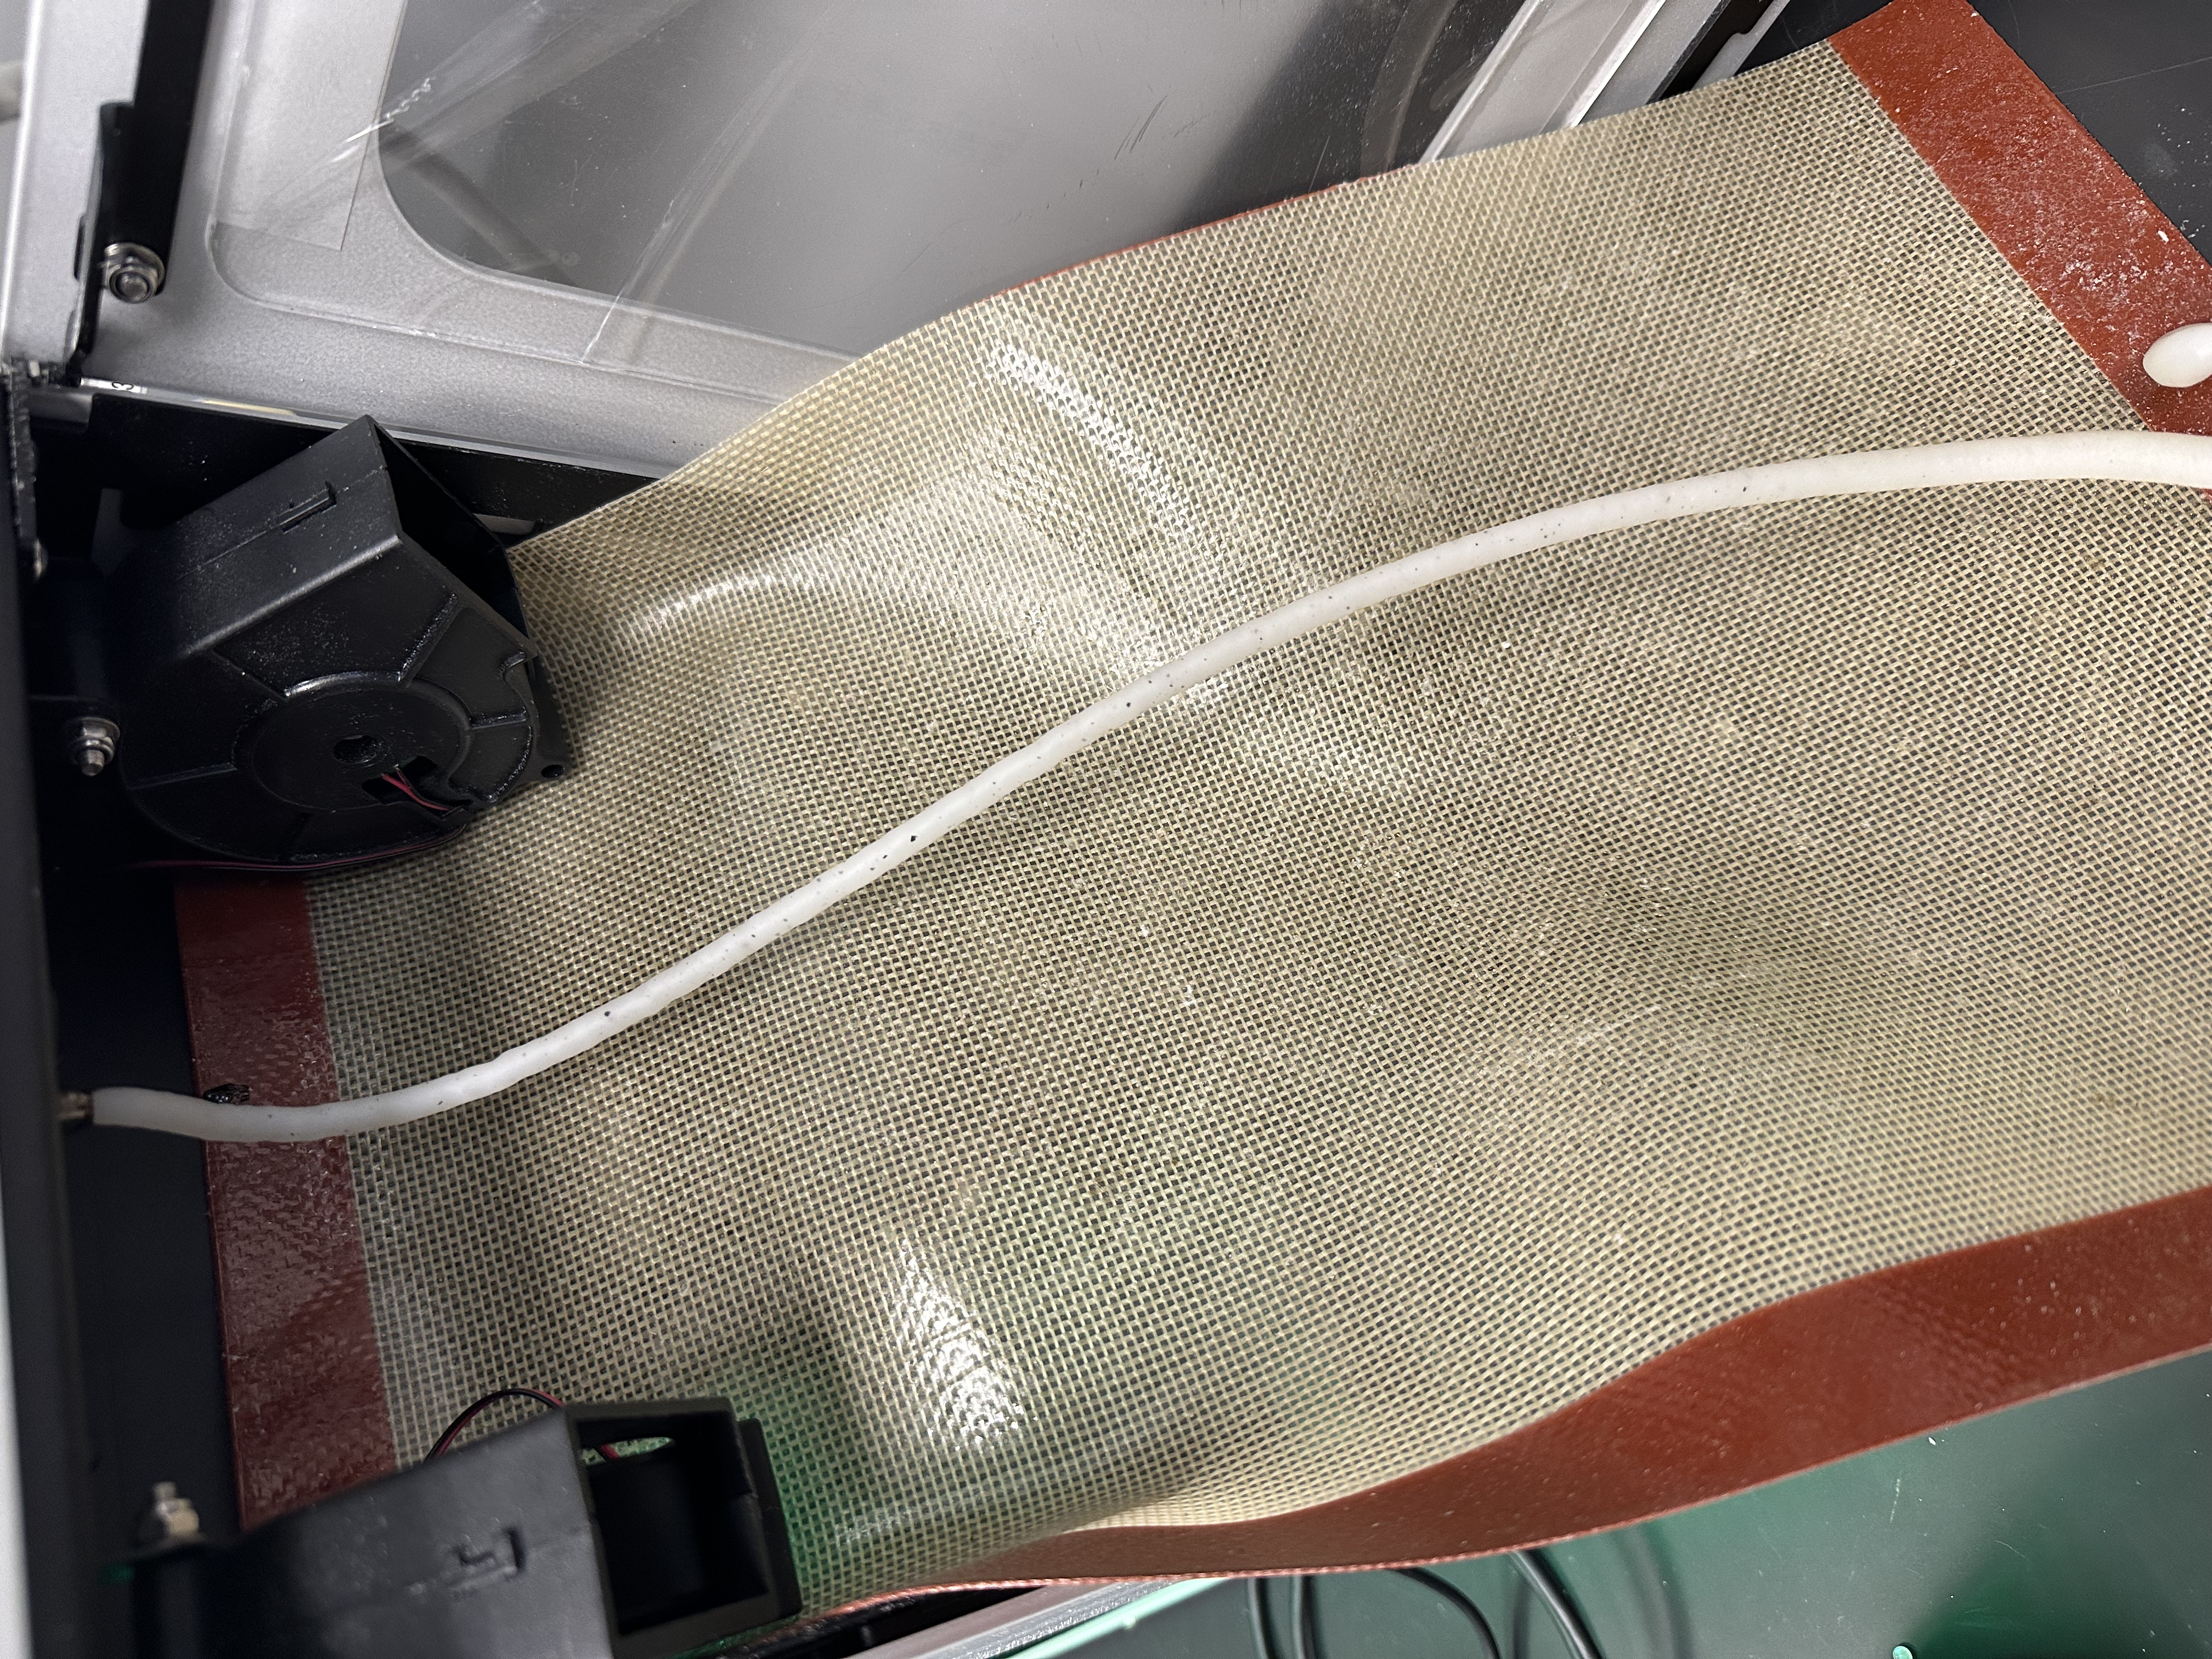
\includegraphics[width=0.5\linewidth]{../figs/discussion/purgingExtruder/dpD2_purge_black_specks.png}
        \caption{Black specks following DP-D2 purge.}
        \label{fig:sec:discussion:extrudingPLCL:pelletExtrusions:purgingExtruder:dpd2BlackSpecks}
\end{figure}

Based on these black specks using DP-D2 as a purging compound, 3Devo customer support suggested replacing the nozzle as this may be contributing to contaminated output. This was now the second time 3Devo customer support suggested a nozzle replacement (see Section~\ref{sec:discussion:extrudingPLCL:pelletExtrusions:addressingFilamentThickness}), which further emphasized the potential need for a new nozzle.

A third extrusion compound, DP-K was also suggested to address the black speck issue.

\paragraph*{Downsides of DP-D2}

As mentioned in Table~\ref{tab:methodology:extrudingPLCL:dpCollaboration:comparingPurgingCompounds}, DP-D2 required HDPE to transition between extruding and purging materials. Subsequent extrusions following DP-D2 purges were found to have HDPE or DP-D2 embedded in the output filament. This is indicative of all purging compound not being extruded when transitioning between materials.

As a result, substantial time and material were required when performing a DP-D2 purge to ensure all material was cleared from the extruder before beginning a new PLA/PCL extrusion.

\paragraph*{Key Takeaways}

The DP-D2 compound appeared to clean more effectively than DP-L, but black contaminant specks were still noticed. Since both purging compounds yielded contaminants, it was hypothesized that the nozzle had contaminants that could not easily be purged, and a nozzle replacement may help.

It was also discovered through trial and error that substantial DP-D2 and HDPE were required to fully clear the extruder and avoid affecting subsequent purges.

\subsection{Felfil Evo Discussion\label{sec:discussion:extrudingPLCL:pelletExtrusions:felfilEvo}}

\subsubsection{Initial PLCL Extrusion Discussion\label{sec:discussion:extrudingPLCL:pelletExtrusions:felfilEvo:initialPLCL}}

\paragraph*{Filament Output}
% a. Can extrude PLCL at proper thickness on 1st pass and faster than 3Devo
% b. First time we've had successul proper thickness PLCL filament

This extrusion attempt showed that the Felfil Evo system is able to successfully extrude PLCL. It can create filament output faster than the 3Devo system, and adjustments to parameters such as heat or RPM are seen more quickly due to the smaller size of the extruder. As a result, the Felfil system should be utilized in refining first-pass PLCL extrusions.

\paragraph*{Monitoring Filament Thickness}

It is a concern of the Felfil system that data such as filament thickness cannot be quantitatively collected. A method for tracking filament thickness as precisely as 3Devo's DevoVision should be employed to adequately compare filement output between the 3Devo and Felfil systems.

\paragraph*{Clumping at Hopper}
% a. Noticed clumping at hopper due to metal wall closest to barrel
% b. Tried using starve feeding method but would need refining/testing
% c. Planned to look into isolating that metal wall section from the raw materials

Throughout this extrusion, significant clumping of material in the hopper was noticed. This was not expected because the hopper is predominantly plastic, so heat from the extruder barrel should be well insulated from the extruding material. However, there are two exposed metal walls that conduct heat from the rest of the extruder. It was found that these walls transfer heat to the material in the hopper and thus prematurely melt PCL pellets, causing clumping. It was hypothesized that the clumping, which led to inconsistent material flow, contributed to the variable filament thickness.

The starve feeder that had been developed for the 3Devo system was attempted to resolve the clumping issue, but this would require additional refinement because the opening for the barrel on the Felfil system is much larger than that on the 3Devo extruder. This allows material to sit in the hopper even if starve feeding is enabled. As a result, it was planned to explore methods of insulating the material from the metal hopper walls to prevent clumping.

\paragraph*{Key Takeaways}

Overall, the Felfil PLCL extrusion was successful in that good-quality filament was extruded at a faster rate than the 3Devo Filament Maker One. Filament thickness was on average near 1.75mm, although there was variability within this thickness.

There is no inherent way to measure filament thickness on the Felfil system, and thus a monitoring system should be developed.

There was also clumping noticed at the hopper while extruding material. As a result, an insulation method should be explored to resolve this.

\subsubsection{PLCL Extrusions with System Modifications Discussion\label{sec:discussion:extrudingPLCL:pelletExtrusions:felfilEvo:modifiedSystem}}

\paragraph*{First-Pass PLCL Extrusions}

With the addition and improvements of the hopper insulator, the pellet clumping was dramatically reduced. Using two hopper insulator pieces with embedded magnets (as shown in Figure~\ref{fig:methodology:extrudingPLCL:pelletExtrusions:felfilEvo:hopperInsulator}) resulted in no clumping throughout the entire extrusion.

It is hypothesized that the clumping led to inconsistent flow rates which in turn caused the variable filament thickness initially recorded. As the hopper insulator improved, clumping decreased, and average thickness approached the ideal $1.75mm$ thickness.

The ability to record thickness measurements through the filament thickness GUI (see Section~\ref{sec:methodology:extrudingPLCL:felfilSystem:filamentThickness}) proved useful in directly comparing extrusion results.

\paragraph*{Second-Pass PLCL Extrusions}

Throughout this extrusion, the filament thickness was initially within ideal bounds and became thinner with time. This transition from proper thickness to thin filament occurred multiple times.

It was noticed that material was sitting in the hopper rather than flowing into the barrel. This is likely caused by the variable thickness and shape of the shredded PLCL regrind. It is hypothesized that making a more uniform regrind shape may lead to a more consistent flow rate and thus filament thickness.

While filament regrind methods were explored (see Section~\ref{sec:methodology:extrudingPLCL:felfilSystem:felfilShredder}), overall shredded filament size was still inconsistent. It is possible that 3D printed parts shred more uniformly than raw filament due to the thickness and continuity of the part. Additionally, a more industrial filament shredder may be required to produce uniform regrind.

\paragraph*{Key Takeaways}

Overall, the adjustments to the Felfil system proved beneficial in producing proper-thickness filament and eliminating clumping at the hopper.

The first-pass PLCL thickness was still variable but had an average thickness of $1.75mm$. The second-pass PLCL became thinner with time. It is hypothesized that a more uniform regrind will lead to proper filament thickness.
